\documentclass[
twocolumn,
%preprint,
rmp,aps]{revtex4-1}

%\usepackage{charter}
%\usepackage{kpfonts}
%\usepackage{mathpazo}
%\usepackage{tgtermes}
%\usepackage{ebgaramond}
%\usepackage{dejavu}
%\usepackage{bera}
%\usepackage{droid}
\usepackage{fourier}
\usepackage{sourcesanspro}
\usepackage{graphicx,CJK,listings,xcolor} 
\usepackage[hidelinks]{hyperref}

\lstset{
    frame=single,
    breaklines=true,
    postbreak=\raisebox{0ex}[0ex][0ex]{\ensuremath{\color{red}\hookrightarrow\space}}
}

\begin{document}
\begin{CJK*}{UTF8}{}

\title{ACE-M2 Progress and Preliminary results, Part 1}
\author{Peter J.~Lu (\CJKfamily{bsmi}陸述義)}
\affiliation{Department of Physics and SEAS, Harvard University, Cambridge, Massachusetts 02138, USA}
\author{David A. Weitz}
\affiliation{Department of Physics and SEAS, Harvard University, Cambridge, Massachusetts 02138, USA}

\date{31 July 2014}
\begin{abstract}
We describe and comment on the progress of preparing, loading and launching
samples for the Advanced Colloid Experiment (ACE-M2), in the Light Microscopy
Module (LMM) within the Fluids Integration Rack (FIR) aboard the International
Space Station (ISS). We have completed several rounds of experiments in June and July,
2014. Here we summarize our findings so far, primarily several operational
developments and lessons learned, with scientific results still largely
forthcoming.
\end{abstract}
\maketitle
\end{CJK*}

\setcounter{tocdepth}{1} 
\tableofcontents

\clearpage

\section{Science on the International Space Station} \label{science-on-the-international-space-station}

\subsection{Why tell our story?} \label{why-tell-our-story}
There are lots of papers, reports, blogs and general writing on space, NASA, and science. So why write more?
\emph{Because very, very few people actually understand how science experiments are conducted, from start to finish, either in the lab, or onboard the on-orbit laboratory of the International Space Station (ISS).}
My aim here to tell the story of how science actually works, for a broad audience:
\begin{itemize}
\item the general tax-paying public who wants to know more about what is going on in NASA
\item NASA staff who may be deeply knowledgable about a small part of the process, but don't get a good overview---and who want to hear directly from the Principal Investigators (scientists)
\item policy folks who want a deeper view of what we do, beyond what can be described in a report
\item the astronaut crew on  we work with, who want a direct line to what we are doing
\end{itemize}

I intend this to be a cross-breed of a blog, textbook, collection of essays and
technical manual. Some of the posts will give the nitty-gritty \emph{in medias
res} narrative of what we are doing on a day-to-day basis. Other entries will
summarize previous knowledge to give an historical context to the work we are
doing. Still others may dive a little deeper into the technical details of the
tools we are using, hardware and software, both to do the science and
communicate its results. I hope to cover a broad range:
\begin{itemize}
\item The scientific background of experiments that precede and motivate ours
\item What we are actually trying to understand in our current experiment
\item How we prepare and characterize our experimental samples
\item What instrumentation and laboratory apparatus we use, on the ground and in orbit
\item The process of packaging and launching our samples to the ISS
\item Conducting on-orbit experiments in collaboration with the astronaut crew
\item The raw data and how we process it
\item How our analysis leads to the scientific story we will tell through papers and presentations
\item Writing a scientific paper
\item Preparing a scientific talk (and possibly its presentation)
\end{itemize}

\subsection{Opening up the process of doing science}\label{opening-up-the-process-of-doing-science}
I aim to be maximally open throughout. This means posting raw data when
feasible, the actual computer code we use for the analysis (and potentially
giving a way for you all to play with the data and code yourself in an
interactive environment---stay tuned), early drafts of the paper as we write it,
and maybe our presentation drafts before they are delivered.

My commitment here is to make as much of our work accessible directly to anyone
to tinker with: open-source software, open-access publications, but also free,
open access to the raw data; even this website itself, hosted on Github, is
completely open---not just the text, but the entire revision history, and the
code that runs it. So please download, play around, make your own modifications,
and let us know through the comments what you think and if you found something
new that we might have missed. This is a different way of doing science that
takes advantage of a lot of the new information-based technologies that were not
available in years past, and the way I think science should be done. I will
elaborate more on the motivation and tools in a later post.
\subsection{Who am I?}\label{who-am-i}
\begin{figure}
\begin{center}
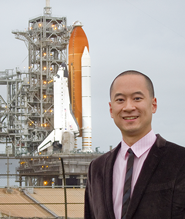
\includegraphics[width=2in]{./images/peterlu_atlantis_launchpad_sm_110707.png}
\end{center}
\caption{Launchpad photo}
\end{figure}

I am a physicist at Harvard, currently serving in a staff position known as a
post-doctoral fellow, meaning I continue to do research after receiving my PhD.
I am funded by {NASA} directly through a research
grant to my official employer, {Harvard University}
(Cambridge, MA), which broadly-speaking supports the scientific aspects of our
work. I also receive some additional support as a subcontractor to assist with
the engineering aspects, helping to develop and test the hardware and software,
of the experiment by working closely with the main NASA contractor,
{ZIN Technologies} (Cleveland, OH). More
information on me and my work can be found on my webpage,
{peterlu.org}. I act independently, and represent
my own views here. Though I am employed by Harvard, they do not control (pretty
much ever) what any of us say or do. NASA, similarly, gives a research grant and
is not able (as much as they sometimes would like) to be able to control what
its funding recipients can say. ZIN is contracted to engineer, deploy and run
complex instrumentation and serves in a technical capacity, and does not appear
to have much of a corporate message to spread beyond NASA.

I do anticipate some fraction of what I write to disagree with the perspectives
of others; if 80\% of the readers agree with me 80\% of the time, then that to
me is a healthy balance that still leaves room for new ideas to develop and be
fleshed out in a congenial manner. If you think I am a little off-base, please
leave some respectful comments and I will do my best to respond in a timely
fashion (though note that I will moderate and delete anything offensive,
off-topic, spam, or irrelevant).

Hopefully we have an interesting and informative journey, and do some great
science along the way!


\section{Why ACE-M2?}\label{why-ace-m2}
We learned a tremendous amount from the series of BCAT experiments conducted aboard the ISS over the past decade. One of the challenges of macroscopic photography, however, is the limited ability to see small features. Observable structures have to be at least a few pixels wide, which means we can image features that have to be tens of microns across, or larger. The particles are a half-micron in diameter, which means that the early stages of phase-separation, or indeed any other process we wish to observe with colloids, are not visible with traditional photography. We see this in our data; we don't see much happening within the first (sometimes many) hours after sample mixing.

ACE allows us to put these same samples under the microscope, where we can comfortably get micron-level resolution, and if everything works out, significantly better. Scientifically, we are able to then watch the structures forming from a much earlier time, when they are smaller, which gives insight into the fundamental mechanisms driving these processes. 

The microscope, however, is a new (to us, at least) facility, and its capabilities on orbit are not well-characterized for our purposes: can we get enough light to the sample to see the particles? What is the range of intensities that we can detect at the camera, with the various filters and dichroics in the system? Will the particles be visible? What is the image quality using different microscope objectives? These parameters all depend on our choice of sample, as well as the hardware on orbit, and the on-paper specifications from the manufacturers are often rather poor guides, as they apply primarily to pristine instruments in a clean, ground-based, stable environment---not reflecting the real-world challenges of flying a vehicle in low-earth orbit.

Therefore, we are launching three categories of samples:
\begin{enumerate}
\item \textbf{Fluorescent dyes in solvent:} these samples establish that we are able to observe fluorescence, using the same fluorophores as are in the colloidal particles, but without any particles. This frees us from having to worry about, for instance, whether the particles are stable, or sediment out, or can be mixed.

\item \textbf{Suspensions of fluorescent colloidal particles in solvent:} these samples allow us to measure intensities of different particle concentrations, with the end-goal of being able to take a sample and identify its density (volume fraction) based on fluorecence intensity, a quantitative use of the microscope. They are also a test of whether the particles survive the launch and can be mixed, and are stable and bright.

\item \textbf{Mixtures of colloidal particles and polymers in solvent:} these samples should exhibit dynamic changes, undergoing the process of phase separation. We should see the formation of structures much as we saw in BCAT, but on a smaller length scale and starting much earlier, with higher-magnification microscopy.

\end{enumerate}

\section{Sample composition charts}\label{sample-composition-charts}
Here are the exact samples we delivered to NASA / ZIN, and are launching to the ISS. All of the samples have the same solvent: 18\% cis-decalin, 22\% tetralin and 60\% tetrachloroethylene, where the percentages are based on masses (not volumes). We have two particle sizes---large (880 nm radius) and small (290 nm radius)---and all have the Cy3-MMA fluorescent dye. We use one polymer, a linear polystyrene with a nominal molecular weight of 11.4M; its concentration is expressed in mg of polymer per gram of solvent.

\subsection{Fluorescent dyes}\label{fluorescent-dyes}
\begin{center}
\begin{tabular}{c|c|c|c}
No. & Name & Dye & Conc. \\
\hline
1 & plu\_ACEM2\_Cy3M1 & Cy3-MMA & 0.048\%\\
2 & plu\_ACEM2\_Cy3M4 & Cy3-MMA & 0.012\%\\
3 & plu\_ACEM2\_DiI1 & DiI & 0.062\%\\
4 & plu\_ACEM2\_DiI4 & DiI & 0.016\%\\
5 & plu\_ACEM2\_DiO1 & DiO & 0.041\%\\
6 & plu\_ACEM2\_DiO4 & DiO & 0.010\%\\
7 & plu\_ACEM2\_solv &  & 0\\
\end{tabular}
\end{center}

\subsection{Colloidal suspensions}\label{colloidal-suspensions}
\begin{center}
\begin{tabular}{c|c|c|c}
No. & Name & Colloid size & $\phi$\\
\hline
8 & plu\_ACEM2\_lg\_40p0 & large & 40.0\%\\
9 & plu\_ACEM2\_lg\_30p0 & large & 30.0\%\\
10 & plu\_ACEM2\_lg\_19p9 & large & 19.9\%\\
11 & plu\_ACEM2\_lg\_10p7 & large & 10.7\%\\
12 & plu\_ACEM2\_lg\_05p2 & large & 5.2\%\\
13 & plu\_ACEM2\_lg\_00p4 & large & 0.4\%\\
\hline
14 & plu\_ACEM2\_sm\_45p0 & small & 45.0\%\\
15 & plu\_ACEM2\_sm\_29p9 & small & 29.9\%\\
16 & plu\_ACEM2\_sm\_19p8 & small & 19.8\%\\
17 & plu\_ACEM2\_sm\_10p1 & small & 10.1\%\\
18 & plu\_ACEM2\_sm\_05p0 & small & 5.0\%\\
19 & plu\_ACEM2\_sm\_00p5 & small & 0.5\%\\
\end{tabular}
\end{center}

\subsection{Colloid-polymer mixtures}\label{colloid-polymer-mixtures}
\begin{center}
\begin{tabular}{c|c|c|c|c}
No. & Name & Colloid size & $\phi$ & $C_\mathrm{p}$ \\
\hline
20 & plu\_ACEM2\_sm\_ps & small & 15.0\% & 0.529 mg/g\\
21 & plu\_ACEM2\_lg\_ps & large & 20.5\% & 0.153 mg/g\\
22 & plu\_ACEM2\_lg\_gel & large & 22.0\% & 0.275 mg/g\\
\end{tabular}
\end{center}


\section{Choosing the sample well layout}\label{choosing-the-sample-well-layout}
We have 30 wells in total, and 22 samples prepared. We distributed the samples
throughout the strips in such a way that we would preserve the broadest range of
scientific observations if we lost a well, or a strip; that is, we sought to
avoid actively placing all of the same types of samples physically near each
other, in case something went wrong.

\begin{figure}
\begin{center}
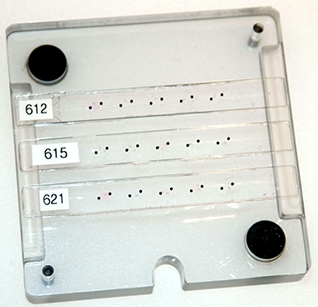
\includegraphics[width=2.5in]{./images/ace_m2_sample_tiles/platter_2104_web.png}
\caption{Sample platter 2104}
\end{center}
\end{figure}

\begin{figure}
\begin{center}
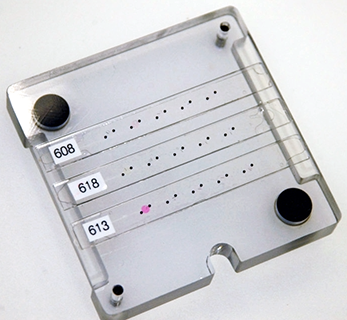
\includegraphics[width=2.5in]{./images/ace_m2_sample_tiles/platter_2105_web.png}
\caption{Sample platter 2105}
\end{center}
\end{figure}

The sample composition chart can be tedious to work with, because it's
effectively just a list of numbers. So to facilitate keeping track of the
different samples and their well locations, I created an icon-based chart. Each
entry in the table has a square icon tile, containing all of the relevant
information on each sample, which can be read at a quick glance.

\subsection{Dye samples}\label{dye-samples}
Dye samples have the name of the dye written in the color of the dye solution
(red and yellow), within the grey circle; the brightest colors represent the
higher concentration (of two), and the faded / lower-saturation text occurs in
samples with the lower concentrations.

\subsection{Colloidal suspensions}\label{colloidal-suspensions}
Each sample has a pie chart showing the volume fraction (out of 100\%) in bright
red. The radius of the circle denotes the particle size. Samples with the larger
(of two) particle diameters have circles that nearly fill the black squares,
where the exact volume fraction is written in text \emph{within} the pie chart.
For samples with the smaller particle diameter, the pie chart is substantially
smaller, and the text indicating the volume fraction resides \emph{outside} the
pie chart.

\subsection{Colloid-polymer mixtures}\label{colloid-polymer-mixtures}
These samples follow the same convention as for the colloidal suspensions;
however, those samples with depletant polymer have a blue triangle at the
lower-right of the square. For samples that are expected to phase separate in a
thermodynamic process known as spinodal decomposition, the blue triangle is
hatched. For samples that are supposed to kinetically arrest into a gel state,
the blue triangle is solid.

\begin{table*}
\begin{center}
\begin{tabular}{cccccc}
Strip & Well 1 & Well 2 & Well 3 & Well 4 & Well 5\\
\hline
\textbf{612} & 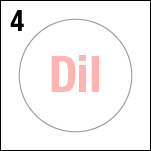
\includegraphics{./images/ace_m2_sample_tiles/sample04.png} & 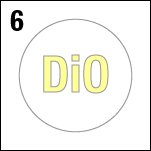
\includegraphics{./images/ace_m2_sample_tiles/sample06.png} & 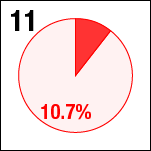
\includegraphics{./images/ace_m2_sample_tiles/sample11.png} & 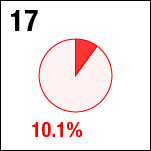
\includegraphics{./images/ace_m2_sample_tiles/sample17.png} & 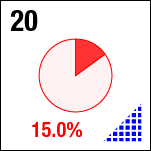
\includegraphics{./images/ace_m2_sample_tiles/sample20.png}\\
\textbf{615} & 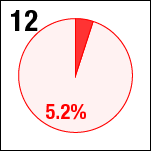
\includegraphics{./images/ace_m2_sample_tiles/sample12.png} & 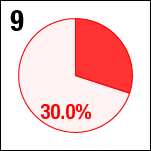
\includegraphics{./images/ace_m2_sample_tiles/sample09.png} & 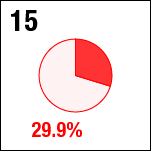
\includegraphics{./images/ace_m2_sample_tiles/sample15.png} & 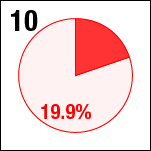
\includegraphics{./images/ace_m2_sample_tiles/sample10.png} & 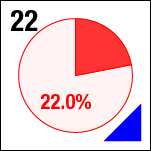
\includegraphics{./images/ace_m2_sample_tiles/sample22.png}\\
\textbf{621} & 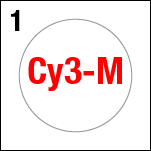
\includegraphics{./images/ace_m2_sample_tiles/sample01.png} & 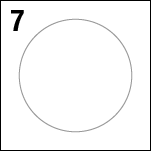
\includegraphics{./images/ace_m2_sample_tiles/sample07.png} & 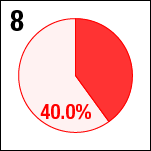
\includegraphics{./images/ace_m2_sample_tiles/sample08.png} & 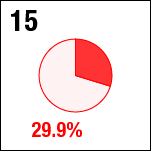
\includegraphics{./images/ace_m2_sample_tiles/sample15.png} & 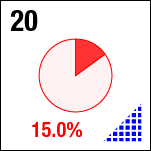
\includegraphics{./images/ace_m2_sample_tiles/sample20.png}\\
\end{tabular}
\caption{Sample platter 2104}
\end{center}
\end{table*}


\begin{table*}
\begin{center}
\begin{tabular}{cccccc}
Strip & Well 1 & Well 2 & Well 3 & Well 4 & Well 5\\
\hline
\textbf{608} & 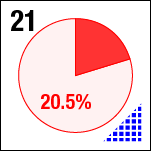
\includegraphics{./images/ace_m2_sample_tiles/sample21.png} & 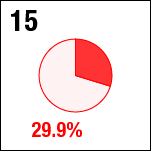
\includegraphics{./images/ace_m2_sample_tiles/sample15.png} & 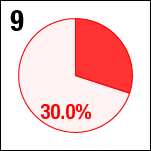
\includegraphics{./images/ace_m2_sample_tiles/sample09.png} & 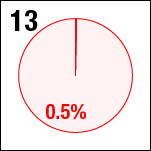
\includegraphics{./images/ace_m2_sample_tiles/sample13.png} & 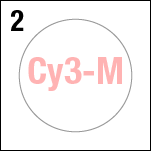
\includegraphics{./images/ace_m2_sample_tiles/sample02.png}\\
\textbf{618} & 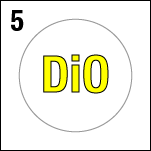
\includegraphics{./images/ace_m2_sample_tiles/sample05.png} & 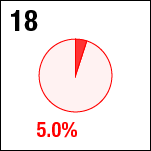
\includegraphics{./images/ace_m2_sample_tiles/sample18.png} & 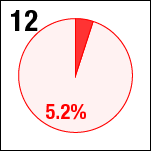
\includegraphics{./images/ace_m2_sample_tiles/sample12.png} & 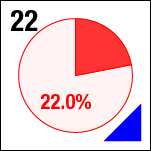
\includegraphics{./images/ace_m2_sample_tiles/sample22.png} & 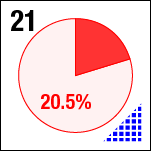
\includegraphics{./images/ace_m2_sample_tiles/sample21.png}\\
\textbf{613} & 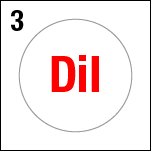
\includegraphics{./images/ace_m2_sample_tiles/sample03.png} & 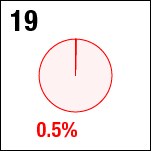
\includegraphics{./images/ace_m2_sample_tiles/sample19.png} & 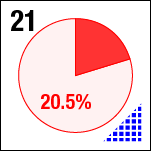
\includegraphics{./images/ace_m2_sample_tiles/sample21.png} & 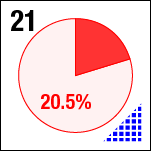
\includegraphics{./images/ace_m2_sample_tiles/sample21.png} & 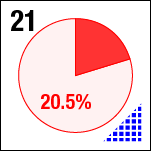
\includegraphics{./images/ace_m2_sample_tiles/sample21.png}\\
\end{tabular}
\caption{Sample platter 2105}
\end{center}
\end{table*}

\clearpage
\section{First day of operations}\label{first-day-of-operations}
We have commenced the first image acquisition in the light microscopy module (LMM) as part of the ACE-M2 experiment. The LMM system is being controlled directly by the Payload Developer (PD), Lou Chesney, sitting at the bank of computer screens that run the control software:
\begin{figure}[h]
\begin{center}
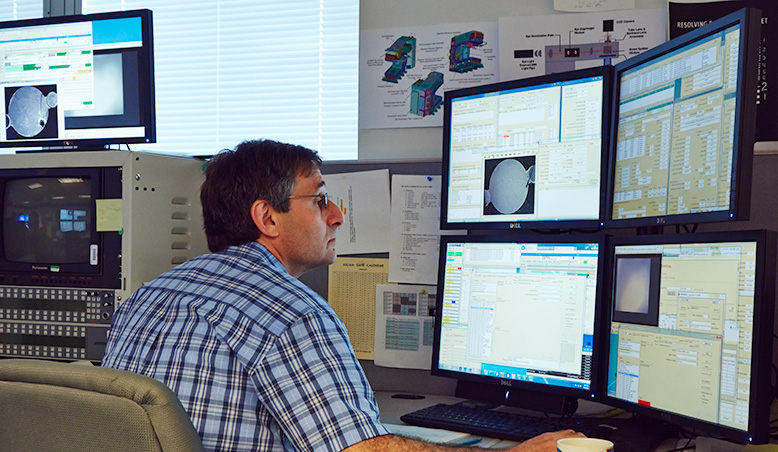
\includegraphics[width=3.1in]{./images/2014_06_04_first_day/140604_ace_tsc_chestney_lou_web.jpg}
\end{center}
\caption{Lou Chesney}
\end{figure}

Because the microscope is onboard the International Space Station, the communications between the commands Lou issues on the ground, and what happens on orbit depends on close coordination with the general communications with the ISS. In particular, there are frequent interruptions of communications and controls, depending on where in its flight path the Space Station is, relative to the geostationery satellites that relay its communications first to Marshall Space Flight Center (MSFC) in Huntsville, Alabama, then to the Telescience Center (TSC) here at NASA Glenn Research Center (GRC) here in Cleveland. The rack officer (RO) coordinates these communications, and integrates the specific timing of operations with the general ISS timeline; this morning, Jim Birchenough is serving in both this role, and as the data management officer (DMO)---overseeing the data downlink so we can live previews and downloaded images---and has his own bank of screens to monitor:
\begin{figure}[h]
\begin{center}
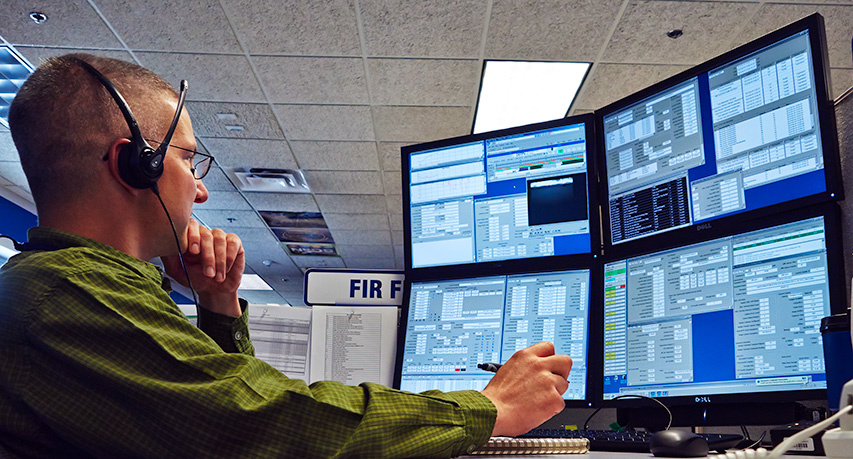
\includegraphics[width=\columnwidth]{./images/2014_06_04_first_day/140604_ace_tsc_birchenough_james_web.jpg}
\end{center}
\caption{James Birchenough}
\end{figure}

After a full 8-hour shift, Lou and James swapped positions with Tibor Lorik (PD) and Amber Krauss (RO / DMO):
\begin{figure}[h]
\begin{center}
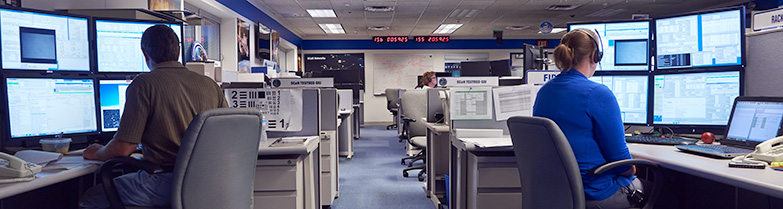
\includegraphics[width=\columnwidth]{./images/2014_06_04_first_day/140604_ace_tsc_tibor_amber_web.jpg}
\end{center}
\caption{Tibor Lorik and Amber Krauss}

\end{figure}


\section{First images from the Light Microscopy Module (LMM)}\label{first-images-from-the-light-microscopy-module-lmm}
We have 15 samples in the holder in this set of experiments, and our first task
is to image all of the samples with the lowest-magnification microscope
objective lens (2.5x). This lens's magnification is ideal for the task, as it
gives an image of each entire sample well. We first use brightfield transmission
illumination (50/50 filter), where the intensity of the image is proportional to
the amount of light passing through different parts of the sample. Thus,
magnetic stir bar appears dark, as it transmits no light, and the glass appears
bright, as most of the light passes through. Bubbles act as mini-lenses, and
therefore are bright in the center and dark around their edges; the light from
the edges is bent toward the center (or focused) by the bubble. These features
are evident in an image of well number 5, containing a phase-separating sample,
as shown in the image on the left.
\begin{figure}
\begin{center}
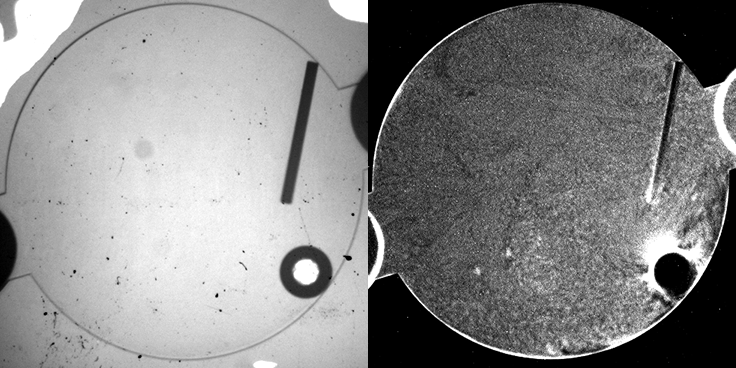
\includegraphics[width=\columnwidth]{./images/2014_06_04_first_day/140604_well5_2p5x.png}
\caption{well 5, 2.5x mag, brightfield transmission}
\end{center}
\end{figure}

The image on the right is the same sample and position, but collected in
fluorescence mode, where the intensity is proportional to the number of
(fluorescent particles). Interestingly, we observe higher concentrations of
particles aggregating around the edges of the sample chamber, the stir bar and
the bubbles. Neither the stir bar nor bubble contain any fluorescent particles,
and like the background glass appear black.

\section{Compositing images to get a higher-magnification view of the entire sample}\label{compositing-images-to-get-a-higher-magnification-view-of-the-entire-sample}
The 2.5x images are good to show the entire sample, but the resolution is
limited. To get a higher-resolution view of the sample, we switch to a
higher-magnification objective lens; however, the tradeoff is that the field of
view is curtailed, and only part of the sample fits into the visible field of
view. Fortunately, the LMM has an automated stage, so that the position of the
sample visible to the microscope can be controlled remotely. As a result, we can
take images in a tile-pattern that cover the entire sample:

\begin{figure}
\begin{center}
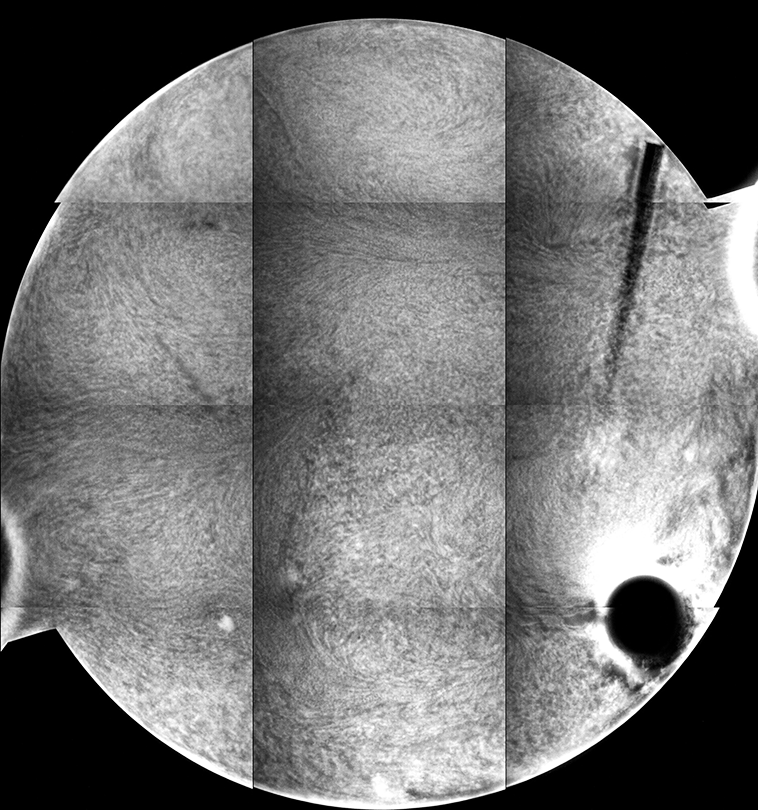
\includegraphics[width=\columnwidth]{./images/2014_06_04_first_day/140604_well5_composite}
\caption{well 5, 10x mag, fluorescence tiled composite}
\end{center}
\end{figure}

The different fluorescence images are the tiled composite image taken at
different depths from the cover slip inside the sample. If you look at the stir
bar, you can see how different parts of the bar come into ``focus'' in the
different images, giving an indicator of the depth within the sample from which
the images are collected.

Each ``tile'' is a bit darker to the left, so that the rectangles representing
each individual 10x image are easily seen. This is a result of uneven
illumination; the samples are illuminated by light from a lamp, which does not
cover the sample evenly (which might be ameliorated by changing internal
microscope aperture settings).

But we have another way we might correct for this problem: a couple of our
samples are fluorescent dye dispersed in a solvent inside identical sample
wells---physically, the intensity of fluorescence should be completely even /
isotropic, so any unevenness in the image should be caused by the illumination.
By taking images under identical conditions of both the phase-separating sample
of interest, and of the even dye solution, we should be able to cancel the
background and see the sample without the effects of the uneven lamp
illumination. So we will be testing this in upcoming operations.

Meanwhile, next stage is to look at higher-magnification, where we seek to
understand the details of small portions of the sample, and see the behavior of
these colloid structures up close.
\section{ACE-M3: Quantitative microscopy}\label{ace-m3-quantitative-microscopy}
Thus far, ACE-M2 has been a resounding success. Every one of the samples which
we have launched appears to work as we expected: dyes are bright, colloidal
suspensions show variations in intensity. But most importantly, we are able to
watch quite clearly the early stages of phase separation, as described in
previous posts. So far, so good; we have a great \emph{qualitative}
understanding of what is happening so far.

Upcoming experiments will look at the phase-separating samples in greater
detail, with hope to quantify the rate of phase separation---something we have
been able to do at larger lengthscales with the BCAT series of experiments,
using photography and some image processing. But what we have never been able to
figure out reliably is the concentration of particles in the two phases after
phase separation. Unfortunately, the photos we take with the camera flash are
not \emph{linear} in relating intensity the image to particle concentration.
Why? Imagine photographing clouds; you can't really tell how thick the cloud
layer is just by its brightness; if a lower cloud passes in front of another
one, even if the total cloud thickness doubles, the light (usually) doesn't fall
by exactly half.

These concentrations after the samples phase separate are important for us to
understand some fundamental physics, test existing theories in a new regime, and
be able to place our samples in the context of other systems. And they cannot be
measured on the ground, where sedimentation may take place---which will
inherently change the measured concentrations. So being able to quantify the
relationship between brightness in the microscope and particle density is
extremely important for the science we want to explore, and something we were
never quite able to do with the BCAT experiments.

ACE, however, uses fluorescence, a process that is linear. If you collect light
from a sample well like we have on orbit, if the particle density is twice, the
total brightness should also be twice. You might recall that we already launched
a series of particle suspensions, which was intended to serve this purpose. We
are looking at that data now, and hopefully that should work. But doing careful
experiments means that we are always happy to run independent controls,
cross-checks, and different systems to verify what we think we are seeing. A
different method to quantify the brightness vs. concentration relationship would
therefore be very useful.

Fortunately, we have been given a great opportunity to send up more samples with
the next round of ACE-M experiments, ACE-M3 which (at the moment) is set to
launch in the fall aboard SpaceX-4. Preparing for this experiment involved a
number of unique challenges:
\begin{enumerate}
\item We were only given the go-ahead a couple of weeks ago, after a bit of begging and pleading to squeeze us on board the next rocket! Fortunately, NASA and the great folks at ZIN agreed to make a little more space. So we had five new samples we could prepare---and only a few days to prepare them.
\item Because of the last-minute nature of the sample prep, we were restricted to the materials that were already approved as safe with a new set of sample cells (slightly different in construction from the ones we use on ACE-M2, but no time to update the loading procedures). But luckily, those materials include dyes that are the same colors as the particles, namely those based on fluorescein and rhodamine.
\item We need the samples we prepare to reflect similar optical behavior as the particles, suspensions and mixtures we already launched with ACE-M2. If they are too different, say involving different filters and lenses, then the results might not apply directly to the system whose physical behavior we want to quantify better on orbit.
\end{enumerate}

\subsection{Sample preparation and
characterization}\label{sample-preparation-and-characterization} 
I chose the rhodamine dyes, for the reason that it is red / pink, and our
particles are pink, so I figured it was a decent place to start. Two samples
with the same fluorescence should be the same color in different lighting
conditions. I then took some rhodamine dye and dispersed in water, and ended up
with a very dark red color, like a red wine, and I could barely see through it.
So it seems like it had way too much dye, and I started diluting it out by
factors of 10. But if we want to control the dye concentration, how can you
assess that? Unfortunately, weighing the dye out is not very accurate. I started
with a few mL of water, but the amount of dye is only a couple of milligrams,
and our balance only reads to 0.1 mg, so the error on the dye concentration is
inherently no better than a few percent.

Moreover, how do we predict what the brightness will be in a fluorescence
microscope? Obviously, we could use a fluorescence microscope, but if that is
the instrument we are testing, we would prefer an independent way to measure the
brightness. The best way would be to use a fluorometer, a specialized instrument
that sends in a beam of light at a user-selectable wavelength (i.e. color), and
then measures the amount of fluorescence emitted. Unfortunately, we don't have
such an instrument, and the ones in the chemistry department are not that
convenient.

\subsubsection{UV-Vis absorption
spectroscopy}\label{uv-vis-absorption-spectroscopy} We do, however, have a UV-Vis absorption spectrometer. This instrument sends
light into the sample one color at a time, scanning over a large range of
wavelengths, and records the amount of light passing through. These instruments
are very carefully calibrated, and ours has a second reference light beam, so
the data it outputs is a very careful, quantitative measure of absorbance. Why
does this help? Because in order for light to be re-emitted as fluorescence, it
must be absorbed at a lower wavelength. And by conservation of energy, doubling
the fluorescence emission will lead to double absorption; it's also a linear
relationship (barring some specific quantum mechanical effects which I don't
expect to be sensitive to). So assessing the peak of the absorption gives us a
way to characterize concentration.
\begin{figure}[h]
\begin{center}
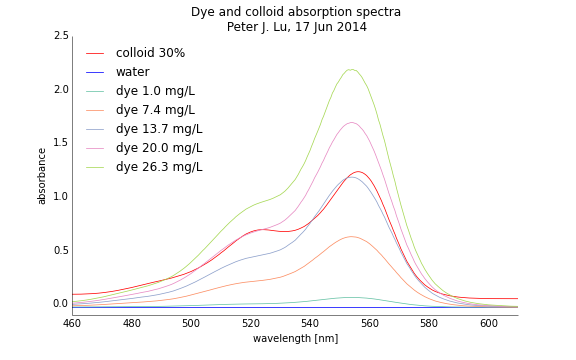
\includegraphics[width=\columnwidth]{./images/2014_06_17_dye/dye_colloid_abs_140617.png}
\end{center}
\caption{UV-Vis spectra}
\end{figure}

First, I ran a sample of just plain distilled water. There should be no peaks in
the absorption spectrum, and it should be basically be flat through the entire
range of wavelengths (460 to 610 nm), as it is colorless---and therefore has no
fluorescence---and transparent. Indeed, this is what I see, shown by the blue
curve in the absorption spectra. I then ran the colloidal sample at 30\% volume
fraction, right in the middle of the range we have on orbit; its spectra has a
nice peak at about 555 nm---which is why the samples appear pink: they absorb
green light, and the absence of green light (e.g. on a color wheel) is pink /
magenta.

Then I ran concentrations of the rhodamine dye; fortunately, the main peak in
the absorption spectrum is very, very close to that of the particles, shown with
the curves in the other colors. You can see how close the peaks are for the
colloids (red) and the dye at a concentration of 13.7 mg/L. This is very, very
fortunate, because it shows how the optical behavior of the dye is an excellent
proxy for the spectral characteristics of our particles!

So by a bit of trial an error, I found the rough dye concentration corresponding
to the brightness of our 30\% colloid sample. Then with some careful sample
prep, I spaced them out linearly over the range of brightness that spans what I
expect the colloids on orbit will (other colored lines in the plot), so we will
learn about the camera and imaging system with parameters similar to what we
will use for the colloids.

\subsubsection{Samples to be launched}\label{samples-to-be-launched}

Here's the final list of samples we submitted to ZIN / NASA:

\begin{center}
\begin{tabular}{c|c}
\textbf{Sample} & \textbf{Dye concentration}\\
\hline
plu\_M3A & 1.05 mg/L\\
plu\_M3B & 7.36 mg/L\\
plu\_M3C & 13.7 mg/L\\
plu\_M3D & 20.0 mg/L\\
plu\_M3E & 26.3 mg/L\\
\end{tabular}
\end{center}

\subsection{Testing linearity}\label{testing-linearity}
\begin{figure}
\begin{center}
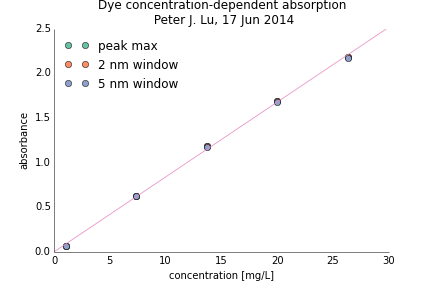
\includegraphics[width=\columnwidth]{./images/2014_06_17_dye/dye_concs_abs_140617.png}
\end{center}
\caption{Absorption vs. concentration}
\end{figure}
To check the linearity of the fluorescence intensity, I measured the height
(absorbance) of each peak at 554 nm, and plotted it as a function of
concentration (from the sample preparation). There are several ways to measure
the peak: reading off the top value, or averaging over a few nm around the
maximum. In all cases, the points fall on top of each other, as seen in the
figure at right, where the different ways of measuring peak height are
indistinguishable. And, critically, the points all fall along a straight line
(purple in the figure), which extrapolates to very close to the origin. These
data show very carefully that the relationship between absorbance---and
therefore fluorescence---is linear with dye concentration, which have similar
spectral characteristics to the colloidal particles we have launched.


This is exactly as we would hope for a good set of standard samples, to use to
then explore and calibrate the imaging system properly, using a different
chemistry while still in the same physical realm (in terms of fluorescence
intensity) that we are interested in for our colloidal samples. So we are very
excited to launch these as a part of the ACE-M3 experiment!

Finally, here is the code from the second plot, with the linear fit to the
{raw data}:
\begin{lstlisting}[showspaces=false,showtabs=false,language=python,basicstyle=\ttfamily\footnotesize,columns=fixed,frame=tlbr,float]
from pylab import *
import csv
import prettyplotlib as ppl

dye_concs_data = []
for row1 in csv.reader(open('peak_summary_130615.txt'), delimiter='\t'): 
    dye_concs_data.append(row1)
header1 = dye_concs_data[0]
water_blank = dye_concs_data[1]
values1 = array(dye_concs_data[2:]).astype(np.float)
concs=values1[:,0]
window5nm = values1[:,2]
linfit = polyfit(concs, window5nm, 1)
fitrange =[0,30]

figure(figsize=(6,4))
for i in range (1,4):
    ppl.plot(concs,values1[:,i],'o')
ppl.plot(fitrange,polyval(linfit,fitrange),'-')
xlabel('concentration [mg/L]')
ylabel('absorbance')
title('Dye concentration-dependent absorption\n Peter J. Lu, 17 Jun 2014')
xlim([0,30])
ylim([0,2.5])
lg= legend(['peak max','2 nm window','5 nm window'],'upper left')
lg.draw_frame(False)
savefig('dye_concs_abs_140617.pdf')
\end{lstlisting}   %  class="language-python"


\section{Science depends on flight ops, which cannot be known ahead of flight}\hypertarget{science-depends-on-flight-ops-which-cannot-be-known-ahead-of-flight}{}\label{science-depends-on-flight-ops-which-cannot-be-known-ahead-of-flight}

\subsection{Putting the cart before the horse}\hypertarget{putting-the-cart-before-the-horse}{}\label{putting-the-cart-before-the-horse}
In the study of literature, there is a literary devive known as \emph{hysteron
proteron}, which colloquially is often termed ``putting the cart before the
horse.'' Alas, the way NASA has structured the way it does science experiments
often has a similar flavor: requiring the answer to be known before the
experiment is performed.

As NASA Principal Investigators (PIs), we are asked to specify requirements for
instrumentation and apparatus that the engineers are then supposed to build. The
problem is, the scientists often spec instrumentation based on what they can get
in the laboratory on the ground, not necessarily what is practical or even
possible to fly on ISS, with its myriad safety, operational, power, mass and
mechanical shock requirements. Similarly, we are told to define scientific
goals, not just a general overview of what we hope to accomplish, but specific
criteria as to what would constitute partial, satisfactory and complete
scientific success.

\textbf{But if we could define specifically what would be successful scientifically, then we would know the answer before asking the question---and there would be little point in doing the actual experiments!}

Moreover, at present, the science office is a subdivision of payloads, which
manage all of the hardware on the ISS. This is a completely different division
than flight operations, the pilots who fly the station and manage its
communication. So inevitably, if science or engineering requirements are defined
from the viewpoint of only one division, it can conflict with what is going on
elsewhere. This is, of course, not a specific problem to NASA, but instead
symptomatic the challenges of working within any large organization.

\subsection{Organizational divisions between science and flight-ops are problematic}\hypertarget{organizational-divisions-between-science-and-flight-ops-are-problematic}{}\label{organizational-divisions-between-science-and-flight-ops-are-problematic}
From a PI standpoint, constraints from flight operations never enter the
specification or definitions of the science experiments. We are told to specify
what we need, which then the science / payloads office coordinates, and has to
try to balance with all of the other experiments and payloads. They are tireless
advocates for our cause, for which we are extremely grateful and have received
very, very generous allocations of crew time and ISS resources. And through this
process we have learned from the many iterations of the BCAT experiment is that
it is invaluable to understand what everyone else's constraints are. Often
times, we would specify that we needed two weeks to run our samples, but if the
flight schedule only had 12 contiguous days available, we would not be able to
use that time, and would have to wait until our nominal requirements (i.e. the
two weeks) were available, even if that would not be possible for many months in
the future. But from our standapoint, 12 days of data now could be worth a lot
more than a ``complete'' set of data months later---especially because all kinds
of things can go awry in the interim (samples may dry out, instruments may get
broken, the Space Station itself may have an operational issue).

Alas, because the normal procedures do not involve science PIs in flight
operations, these types of tradeoffs are not ordinarily presented to the PI, and
instead are negotiated among several constituencies within NASA, who may not
have the background to make the decisions that are best for the science.
Conversely, unless the PIs have been involved in several successful flight
experiments and have worked with the different NASA branches, it's unlikely that
they understand the panoply of constraints that flight on orbit imposes, so it
is hard for them to weigh the practical factors.

As a result, we do the best job we can to suggest what we \emph{a priori} feel
is a reasonable operational plan based on our best guesses as to how the
apparatus will perform, with full awareness of the wisdom of Prussian (German)
field Marshal Helmuth Karl Bernhard Graf von Moltke dictum that, roughly
translated, that ``no battle plan survives first contact with the enemy.''

\section{ACE-M2 first-round flight ops main goal: define and characterize operational capabilities}\hypertarget{ace-m2-first-round-flight-ops-main-goal-define-and-characterize-operational-capabilities}{}\label{ace-m2-first-round-flight-ops-main-goal-define-and-characterize-operational-capabilities}
The main point of the first runs of the ACE-M2 experiment are to image all of
the samples and see if we can actually observe them. If we can't image any
sample in the microscope, then obviously there won't be much use for future
operations. Fortunately, in general we were able to acquire good images of all
of the samples, which I describe in greater detail in a {later post}.

Once this basic ability to image samples has been established, the main objective is to understand the capabilities of our system. This not only includes the physical aspects of the optical system, camera and other instrumentation, but the amount of time different operations actually take when a human is operating the LMM setup amidst all of the mayhem onboard the ISS itself.

\subsection{Optical capabilities: exploring objectives}\hypertarget{optical-capabilities-exploring-objectives}{}\label{optical-capabilities-exploring-objectives}
The LMM is equipped with several microscope objective lenses: 2.5x, 10x, 20x and
40x air, and the 63x and 100x oil-immersion objectives. There are several filter
sets, though we use the Texas Red set for almost all of our samples, whose
spectra we checked before launch so that they were compatible with the dyes we
use in the particles. There is a single CCD camera, made by a company called
QImaging, that uses the Sony ICX285 CCD chip that has been a workhorse for the
entire industry for the first decade of this century, though more recently
surpassed by much better imaging technologies.

\subsubsection{2.5x air: sample surveys}\hypertarget{x-air-sample-surveys}{}\label{x-air-sample-surveys}
Using the lowest-magnification objective, the 2.5x air, we survey every well at
the beginning of each full experiment, with both bright-field and fluorescence,
to check on the status of the sample and see quite generally what is going on,
i.e. the location and density of the particles. This objective lens has a very
large depth of field, encompassing the entire sample well, giving us a very good
overview of each sample. These images also form part of the safety checks at the
beginning and end of each experiment, to make sure for example that the wells
are all intact, not leaking or broken, etc.

\subsubsection{10x, 20x and 40x air: sample details}\hypertarget{x-20x-and-40x-air-sample-details}{}\label{x-20x-and-40x-air-sample-details}
Perhaps the most important objectives are the medium-magnification air
objectives. These allow us to zoom into particular areas in the sample, and get
a more detailed view. In general, the quality of the images appears to be best
with the 10x, and good with the 20x and 40x.

\subsubsection{63x and 100x oil: highly disappointing}\hypertarget{x-and-100x-oil-highly-disappointing}{}\label{x-and-100x-oil-highly-disappointing}
On paper, the 63x and the 100x should give the highest-quality views, because
they at least double the \emph{numerical aperture} of the air objectives; that
is, they should have roughly double the resolution, so that features that are
visible but blurry at 40x should be sharper and more clearly defined, with
better contrast, with the 63x lens.

These two objectives require the addition of immersion oil, a droplet of which
is added by the crew as the samples are loaded. We did a number of different
tests, looking at the same areas with different objectives. Surprisingly---and
not in a good way---the image quality is invariably worse with the
oil-immersion, higher-magnification objectives, than with those that are
air-based. This is backward, and should not happen, and demonstrates that
something is wrong with the current configuration of the microscope on-orbit.
Engineers at ZIN are working on this issue, so stay tuned.

But from a practical standpoint, there is no reason for the immediate future to
incorporate any of the oil-immersion objectives. This has the collateral benefit
that no oil then need be added by the crew members, or manually moved via the
objective to different sample wells, giving greater flexibility to the imaging
of different sample wells.

\subsection{Timing individual operations}\hypertarget{timing-individual-operations}{}\label{timing-individual-operations}
Once the objectives have been selected and we understand how they can best be
deployed to give the images we want, the major task to understand how long
different operations actually take:

\begin{itemize}
\item starting up the LMM inside the FIR rack
\item loading the sample
\item moving the microscope stage to the right positions on the samples
\item establishing the distance between the objective lens and the sample coverslip
\item adjusting imaging parameters on the camera to acquire good images
\item saving and downlinking image data
\item shutting down the rack
\end{itemize}

While we have estimates for how long these operations take on the ground, things are often quite different on orbit. And establishing the timing is \emph{absolutely critical} for planning future operations, all of which must happen in the context of a competition for resources like crew time, machine time, operator time, power, etc.

\subsection{Meshing with the ISS timeline and infrastructure: LOS}\hypertarget{meshing-with-the-iss-timeline-and-infrastructure-los}{}\label{meshing-with-the-iss-timeline-and-infrastructure-los}
One of the major differences between doing experiments on the ground, in a
well-controlled, isolated (university) research laboratory, and the ISS, is the
number of other things happening at the same time. In our labs, there may be a
few people walking in and out of the room, but generally things are still,
power, light, temperature, gases and water are continuously available, and
mechnically the building is stable in the absence of, say, high winds or a major
rainstorm. Almost none of those factors is true on orbit; the ISS is a flight
vehicle, and flies around the earth in orbit, traversing the planet every couple
of hours.

The ISS communicates with the ground via a network of geostationary satellites.
Unfortunately, this network does not cover the entire earth's surface, so that
every few hours (and often more frequently than that), the Station loses
communication, during events known as ``Loss of Signal'' or LOS. During this
time, we cannot access our experiment at all, so either it is running something
in an automated fashion that we can script ahead of time, or it must sit there
until communications are re-acquired.

So not only is the total time relevant for each operation, but complex
experiments must be broken down into a series of smaller sequential operations,
either that execute remotely during an LOS event (ideal, because then we don't
lose any time), or must be robust to being interrupted and (re)started again at
a later time.

\subsection{The human factor: reproducibility and robustness}\hypertarget{the-human-factor-reproducibility-and-robustness}{}\label{the-human-factor-reproducibility-and-robustness}
Finally, the operators on the ground work very hard to collect our data, taking
8-hour shifts at the console controls. They have a wide range of scientific
background, so that we must be very precise in specifying procedures for data
collection and documentation. Moreover, the procedures have to be simple and
reliable enough to be executed without error by an operator working all day,
even as she gets more tired and might overlook something.

\section{Major results from the first run: a flight-ops plan for upcoming experiments}\hypertarget{major-results-from-the-first-run-a-flight-ops-plan-for-upcoming-experiments}{}\label{major-results-from-the-first-run-a-flight-ops-plan-for-upcoming-experiments}
So the most important results from the first run are operations related, once we
established we can image all of the samples. These procedures allow us to
determine what to measure going forward, within the envelope of the resources
that we have. After four 48-hour days to survey all of the samples, the
remaining time will focus on the handful of colloid-polymer mixtures (samples
20, 21 and 22), and imaging them over time. We therefore expect to do the
following for each sample, which based on the first-run operations will feasibly
fit into the timelines we have requested:

\begin{enumerate}
\item Image all wells with 2.5x air objective. This is fast, easy, simple and gives on overall status check for safety and scientific reasons.
\item Create full tiled images of the entire well with the 10x air objective. This is a fast operation that gives us a properly-detailed assessment of each sample of interest; thus far, this lens arguably gives us the best images.
\item Zoom into selective areas and image with the 20x and 40s air objectives. This allows us to focus in more on the evolution of microstructure, guided with the overall tilings from the 10x.
\end{enumerate}

You will see this structure going forward for the observations of time-dynamics
of these colloid-polymer mixtures. Note that this specific set of steps would
\emph{never} have been developed from entirely ground-based studies. Instead, we
developed these procedures based on real experience aboard the ISS.


\section{ACE-M2 first-round flight operations: major milestones achieved}\hypertarget{ace-m2-first-round-flight-operations-major-milestones-achieved}{}\label{ace-m2-first-round-flight-operations-major-milestones-achieved}
With ACE-M2, we sent up almost two dozen new, different samples, and did not
know \emph{a priori} if they would mix properly on orbit, how they would look in
the microscope, or whether we could observe their dynamics with the
instrumentation and constraints we have. After the first round of on-orbit
flight operations, we have a number of significant milestones---that we can mix,
load and image the samples; and that we now have flight operations procedures
that will give us good data going forward, within the envelope of our resources.
Over two 48-hour continuous runs (run 1 was 4-6 June 2014; run 2 was 18-20 June
2014), we were able to examine all of the samples (except for the well that
broke). Because we looked at different racks over each of these runs, I am
combining my discussion of the results treating this as one ``round'' of the
experiment. I will describe a few of the results from the samples that we have
thus far learned, in addition to everything else. As with most interesting
science experiments, the answers beget new questions, which is why this is an
exciting project to work on!

\subsection{Samples can be mixed and
imaged}\hypertarget{samples-can-be-mixed-and-imaged}{}\label{samples-can-be-mixed-and-imaged} As we now know from the first images, the mixing and optics are working well, so we can take
images and see all of the samples well. This is a major success and demonstrates
overall the samples are good, and that there is no obvious show-stopper
preventing us from gathering good data from our samples.

\emph{For reasons that I will elaborate upon in a later post, we are still coming up with a system to label and organize all of the image data, so this summary of results will wait until that process is finished before I add the processed images.}

\subsection{Dye samples}\hypertarget{dye-samples}{}\label{dye-samples}
We can image the fluorescence from all of our dye samples, using the Texas Red
and FITC filters, as appropriate. We don't see any structures in these samples,
so everything is as we expect. The field of illumination is not even, with sever
vignetting near the edges for the lowest magnifications. These samples which we
know to be spatially uniform might therefore provide a way to correct for
inhomogeneous illumination.

\subsection{Colloidal
suspensions}\hypertarget{colloidal-suspensions}{}\label{colloidal-suspensions} We can observe different levels of brightness for different volume fractions in
the simple particle suspensions. Ultimately, we want to be able to calibrate
overall brightness with volume fraction, so these samples will hopefully provide
a calibration mapping between image intensity and colloid volume fraction. This
is critically important to the science, and a major advance of the ACE
experiment over, say, previous BCAT iterations. We have always been interested
in measuring the volume fraction after phase separation is complete, but cannot
do so on the ground (because the phase separation process is different in
microgravity, which is why we do the experiment in the first place!). Being able
to measure that with ACE in our phase-separating samples would be a major
advance.

\subsubsection{Science is
serendipitous}\hypertarget{science-is-serendipitous}{}\label{science-is-serendipitous} Even when a sample may ``fail'' by our pre-existing criteria, we can still learn
interesting things, and turn that into a success by thinking along different
lines. One of the colloidal suspension samples appears to have had a stir bar
stuck in a dense suspension, very likely because the stir bar happened to be
stuck in a place around which colloid sedimented densely, preventing the bar
from being freed later on orbit. However, we know both the starting volume
fraction of the sample throughout the whole sample well, and the fraction of
that well occupied by dense colloid that sedimented. This allows us to estimate
the volume fraction, which we expect to be near to the hard-sphere glass
transition volume fraction of 58\%. That would give us an additional volume
fraction point on our calibration curve---one which is not possible to create
otherwise, because you physically could not load a colloidal suspension at that
density! Sometimes, even an initial failure can give you data you could not
otherwise acquire!

\subsection{Colloid-polymer
mixtures}\hypertarget{colloid-polymer-mixtures}{}\label{colloid-polymer-mixtures} We have three colloid-polymer mixture sample classes. One is a phase-separating
mixture of small particles and polymer; another is a phase-separating one with
large particles; and the third is an arrested gel (at least on earth) that
involves large particles and polymer.

\subsubsection{Phase separating
samples}\hypertarget{phase-separating-samples}{}\label{phase-separating-samples} Initial observations indicate that the mixing is sufficient, and we can watch
the evolution of structures in these samples over several days. The timescale is
quite appropriate for the ACE experiment: samples change over hours or days,
making useful the collection of similar sets of data over the course of days to
weeks. They are not changing so fast that we will miss the activity during
sample mixing and loading into the LMM; nor are they so slow that no activity is
discernable during our runs. This is all very good news.

\subsubsection{Gel sample}\hypertarget{gel-sample}{}\label{gel-sample}
Moveover, after waiting several weeks, we see the formation of stable colloidal
structure which may or may not be kinetically arrested; we are eagerly awaiting
new data on this particular point.


\section{ACE-M2 Run 4: comparing time evolution among wells with the same sample}\hypertarget{ace-m2-run-4-comparing-time-evolution-among-wells-with-the-same-sample}{}\label{ace-m2-run-4-comparing-time-evolution-among-wells-with-the-same-sample}
The main purpose of Run 4 for ACE-M2 is to observe the time evolution of phase
separating samples in platter 2105, which has five wells all with sample 21 plu\_ACEM2\_lg\_ps, the
phase-separating colloid-polymer mixture using the larger particles. We know
from the comprehensive survey in Run 2 that these samples visibly phase
separate, so the goal is to look at the different wells and see if they all
behave the same---as they should, given that the sample is identical. There may
be some minor variations due to slightly different bubble size and/or mixing by
the crew, but overall we expect similar evolution and structure.

\subsection{Strips 608 and 613: samples A1, C3, C4 and C5}\hypertarget{strips-608-and-613-samples-a1-c3-c4-and-c5}{}\label{strips-608-and-613-samples-a1-c3-c4-and-c5}
As we are standardizing on procedures, we first image the entire well with a 10x
composite tiling at a depth of 80 microns, which for samples A1, C3, C4 and C5
are pretty much the same:
\begin{figure}
\begin{center}
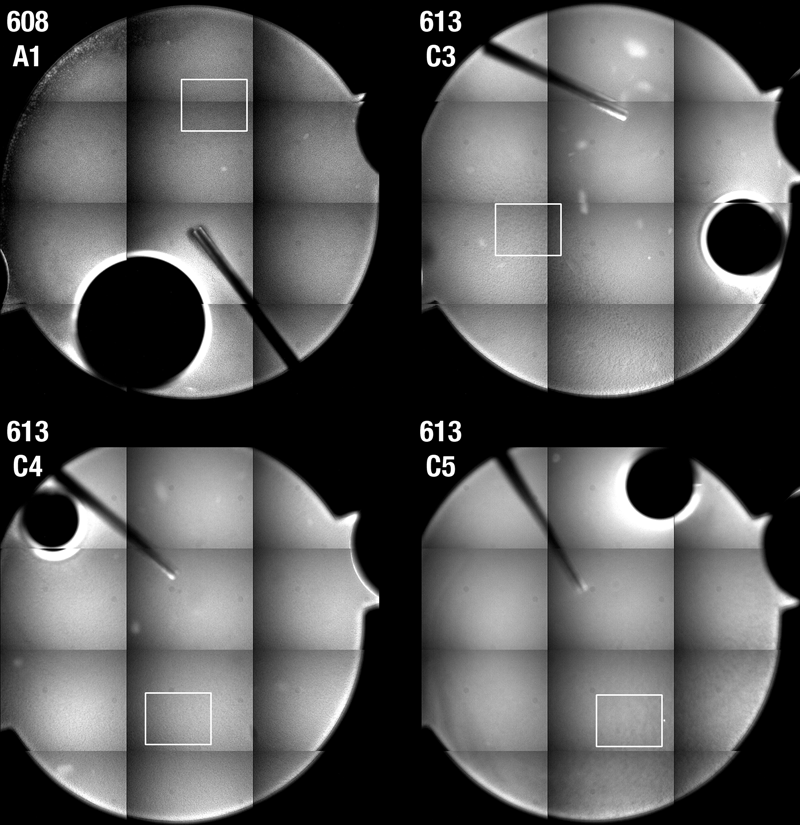
\includegraphics[width=\columnwidth]{./images/2014_07_14_ace_m2_run4/A1_C345_80uM_run4_web.png}
\end{center}
\caption{four similar phase-separating samples A1, C3, C4 and C5}
\end{figure}

The wells look mostly well-mixed, with a small amount of phase separation
visible as the texture in the images develop. But the feature size of the
separation is similar in all wells, so this is suggests we are being consistent
in loading, mixing and imaging.

\subsection{Strip 618: sample B5}\hypertarget{strip-618-sample-b5}{}\label{strip-618-sample-b5}
By contrast, sample B5 is completely different. There is some structure forming,
which is at a much larger length scale: uniformly far more coarse, throughout
the sample well.
\begin{figure}
\begin{center}
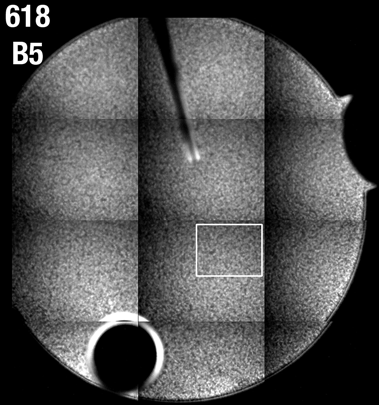
\includegraphics[width=\columnwidth]{./images/2014_07_14_ace_m2_run4/B5_80uM_run4_web.png}
\end{center}
\caption{different-looking phase-separating sample B5}
\end{figure}

This differs significantly from the other four wells, and there is no obvious
scientific reason that we should expect this. Hopefully we will be able to
resolve this mystery with more data as it is collected.
\section{Data organization cannot be defined before the experiment runs}\hypertarget{data-organization-cannot-be-defined-before-the-experiment-runs}{}\label{data-organization-cannot-be-defined-before-the-experiment-runs}
We have received hundreds of images from the first three runs, and the current
fourth run, from ACE-M2 over the past few weeks. Yet I haven't been posting very
much in the way of analysis. Why? It's not because I haven't received or looked
at the image, but because of another fundamental challenge: how the data is
organized and presented to us (as the PIs) from NASA and ZIN, who are running
the experiment.

\subsection{We don't know ahead of time what data we will take}\hypertarget{we-dont-know-ahead-of-time-what-data-we-will-take}{}\label{we-dont-know-ahead-of-time-what-data-we-will-take}
NASA typically has an engineering culture, where goals are specified, often with
mind-numbing specificity, and criteria for progress and success defined. This is
fine when the task to be accomplished can actually be defined ahead of time, as
in the design, engineering, fabrication, launch and operation of a piece of
equipment. But this mentality is a less convenient fit for scientific
experiments, where the main objective is to learn something \emph{newe} about a
scientific phenomenon. This is especially true in our little corner of
soft-matter physics, where we do experiments quickly, change things rapidly in
response to what we see, then do another experiment---much like the ``fail
quickly'' mentality of Silicon Valley startups.

\subsection{Lots and lots of potential data we could collect}\hypertarget{lots-and-lots-of-potential-data-we-could-collect}{}\label{lots-and-lots-of-potential-data-we-could-collect}
To that end, we launched a wide range of samples of different kinds of
materials: dyes, suspensions of colloids in solvent, and colloid-polymer
mixtures that undergo phase separation and gelation. The LMM microscope has
several objective lenses (2.5x, 10x, 20x, 40x, 63x, 100x) and several modes of
imaging (bright-field, fluorescence) and the fluorescence mode has several
filters to excite and detect at different wavelengths. And within each sample,
there are several different locations that we could image, and a variety of
depths. So there are thousands upon thousands of possible choices we can make to
collect an image from the sample.

This tremendous flexibility makes ACE a potentially powerful experiment, but at
the cost of simplicity. With BCAT, we had a single view (fill the frame with the
sample), and only one sample at a time---which takes several weeks to run. The
data involves a single time series of a few hundred images, which get nicely
zipped up and posted weekly by our extremely talented and hardworking
point-woman at ZIN, Cathy Frey. Nonetheless, while the BCAT data is now easy to
organize, it took several years and probably a dozen runs before we got our
stride in what images to collect. With ACE, the problem is probably two orders
of magnitude more complex!

\subsection{Existing data structure therefore represents a best-guess by engineers years in advance}\hypertarget{existing-data-structure-therefore-represents-a-best-guess-by-engineers-years-in-advance}{}\label{existing-data-structure-therefore-represents-a-best-guess-by-engineers-years-in-advance}
At the moment, there is a relatively byzantine file-folder structure that places
images from data sets in a tree labeled by a number of things, including date,
experiment number, and objective lens. We didn't know what samples we were going
to launch until a few months before delivery, because we need always to keep the
experiments as up-to-date as possible, to make sure we are using the most
advanced sample preparation and to tie into the science that is actually
interesting \emph{now}. As convenient as it is for the bureacrats, specifying
these things years in advance only guarantees that the results are not
interesting to anyone.

By contrast, the instruments (e.g. the LMM) must undergo years of development
and testing before launch, and simply cannot wait until we have samples ready,
because of all of the constraints in engineering that operating on-board the ISS
requires. So the engineers who build the hardware and design the software and
protocols \emph{cannot possibly know} what the actual experiments will be. This
is the challenge of the long-latency structure of operating experiments in
microgravity (and is absolutely not endemic to NASA; ESA has exactly the same
issues, as do other agencies).

All of this is \textbf{absolutely not a criticism} of anyone or any part of the
process. It's just a big challenge that we must overcome to be successful in
doing real, dynamic, new science onboard the ISS. Nevertheless, this leads to an
important truth:
\begin{center}
\rule{\columnwidth}{0.5pt}

\textbf{The organization, transmission, storage and curation of data is
a fundamental part of doing both proper engineering and actual new science onboard
the ISS, which is almost never mentioned, and people never really think about.}
\rule{\columnwidth}{0.5pt}
\end{center}

It's basically assumed that, by some magical process, whatever data the PI wants
will magically appear online, which they should hurry up and download, analyze,
and get results back \emph{this week} to send results back to everyone in the
weekly science summary.

For any given week, I can tell you what the science summary is: we got data, and
we are trying to figure out what we are looking at, and if it's correct. Jumping
to any more rapid conclusions---or, worse yet, trying to spread the message in
public, to the press, or via social media---is courting cold-fusion disaster.
Yes, the news cycles are quick, and people want an instant reaction or result
spread immediately.

\emph{Unfortunately, the process of actually doing science is limited by human brainpower, and all evidence suggests that social media makes us if anything stupider. I certainly haven't become faster at fundamental understanding due to the advent of social media, though others may be more talented.}

Nonetheless, the process of understanding what is happening quickly improves
with experience. We had a good idea what we were seeing by the third round of
BCAT phase-separation samples (though recent data from BCAT-KP is fundamentally
different---therefore quite exciting---but then we are back to not know what is
going on---and that's where the fun is). But ACE is a complex experiment where
everything is new, and the main reason we launched so many different kinds of
samples is that we didn't know what to expect!

And this is where the data organization is a big challenge, basically of the
chicken-and-egg type. We don't know what images we are going to collect, so we
can't specify how it should be organized. So we get what the engineers thought
would work best, basically what is logical from a collection standpoint, which
almost by definition is not going to be ideal for the science. So it is an
enormous task to sort everything out, and validate the data: how do I know that
an image I open up on my computer is from the right sample, with the combination
of parameters (lenses, camera settings, position, depth, etc.)?

Ultimately, there needs to be a \emph{combined, close effort between the
science-based PIs and engineers (in concert with operations)} to define the
right procedures for collecting, labeling, and transmiting the right data from
ISS to NASA on the ground and ultimately to us in the lab who will analyze the
data. To do this, we need first to understand the challenges of the existing
systems, as well as the scientific requirements, then develop a proposal for
moving forward. \textbf{And this cannot be done before actually acquiring and
receiving significant data from ISS; there is no way to do this ahead of time!}

\section{Limitations of the current data organization}\hypertarget{limitations-of-the-current-data-organization}{}\label{limitations-of-the-current-data-organization}
The current way data is collected and stored on LMM has several fundamental
issues which must be resolved before the set of images collected onboard ISS
becomes usable experimental data. Just as the raw voltage levels from each pixel
of the camera need to be assembled into a digital image, those images must be
assembled into well-organized, well-documented collections in order to be at all
useful. And those images must be connected

\subsection{Metadata is not stored with the images}\hypertarget{metadata-is-not-stored-with-the-images}{}\label{metadata-is-not-stored-with-the-images}
The \emph{metadata} of each image, including the camera settings (exposure,
gain, black-level offset), microscope settings (objective lens, filter,
illumination), sample location (sample well, and x-y-z position within it) are
not stored in the image itself, for example in metadata fields within a TIF
image (which could easily defined to contain this). The software that writes the
image to disk does not incorporate any of this information with the image
itself. So there is no ``self-documentation'' of each image, which represents a
good practice in general, especially when we have so many images. Anything else
quickly becomes prone to error.

\subsection{Some information is stored in the directory}\hypertarget{some-information-is-stored-in-the-directory}{}\label{some-information-is-stored-in-the-directory}
Right now, which sample well and platter, which can be mapped 1-to-1, then the objective, and
the depth within the sample, are each stored in various directories / folders,
within which the images for each day are sorted. There are additional levels of
folders for the timing (seconds elapsed since experiment was run) and an
experiment number defined by the operator.

\subsection{When a number is assigned to an experiment, and what an experiment includes, varies significantly}\hypertarget{when-a-number-is-assigned-to-an-experiment-and-what-an-experiment-includes-varies-significantly}{}\label{when-a-number-is-assigned-to-an-experiment-and-what-an-experiment-includes-varies-significantly}
As we are defining what data to collect, what amount corresponds to a new
experiment number has varied both over time, and between operators. So data gets
put into new experiments in some places in a way that is not the same as other,
ostensibly identical data.

\subsection{File names are basically all the same}\hypertarget{file-names-are-basically-all-the-same}{}\label{file-names-are-basically-all-the-same}
This is a significant problem when it comes to data organization. A typical
filename is {\tt 00001\_00000.tif}, and in fact remains the same for different
samples, and different days. Thus, if a file is moved out of its directory, all
information is lost and it cannot be checked to see where it came from.

Moreover, when we look at the evolution of samples over time, having the same
exact filename means I cannot simply drag images from the same place, objective,
depth, and settings from successive days into the folder, but have to rename
each one individually, without direct access by the operator who collected the
images. This makes any form of automated analysis impossible, and even manual
analysis is a challenge to even keep track of what images I am looking it.

Of course, there was no obvious way to specify how the engineers could have
added the right information ahead of time, not knowing what samples would be,
how we would look at them, etc. etc. Probably the best they could have done was
to generate a random alphanumeric code as part of each image's filename, which
could then be later correlated, but that would not have been much of an
improvement.

\emph{Instead, what we need is a comprehensive plan to organize the data we have
collected, which involves close cooperation between us on the science / PI side,
the engineers who designed the hardware and wrote the software, and the
operators who actually collect the data.} So here's the current proposal for how
to move forward, which I and Louis Chestney (who wrote the software and
collected a lot of great data) came up with:

\section{How we plan to organize things}\hypertarget{how-we-plan-to-organize-things}{}\label{how-we-plan-to-organize-things}
Unfortunately, there is no perfect, or even optimal way, to organize the data,
involving thousands of images from dozens of amples on dozens of days of
operations. We have a number of constraints, conceptual and practical, that have
to be addressed.

There is always a tension between organizing the data in a way that is best for
the subsequent analysis, and one that reflects the history of how it was
collected. The problem is that the history can be haphazard, in our case jumping
around to take different samples at different settings. And the analysis is
never defined until basically it's done, and we don't want to have to do this
process more than once.

Moreover, there is a limit to the number of characters that fit comfortably
within a filename before some of the computer systems that handle the files get
unhappy (thank you IBM and Microsoft from the 1980s for this horrid legacy).

So for the most common / redundant parts of the metadata, such as well, sample
number, and objective, we use folders to hold that information. This is more for
convenience and making it easy to check / validate the images, as well as
consult historical records. For things that change each run that are important
(e.g. sample position, date), we put that in the filename, which also serves to
document . And for the less-important things (camera settings), we keep that
information in a separate database of sorts.

\subsection{Folder organization}\hypertarget{folder-organization}{}\label{folder-organization}
The first set of folder hierarchies correspond to what sample well we are
looking at, since that is the way the raw data is actually collected (i.e. at
one well at a time). So the first three levels of directory structure [with
examples] are :

\subsubsection{Platter [{\tt platter\_2105}]}\hypertarget{platter-platter2105}{}\label{platter-platter2105}
We have two platters (2104, 2105) in ACE-M2, and one platter with our samples
(2109) in ACE-M3.

\subsubsection{Strip [{\tt strip\_E\_618}]}\hypertarget{strip-stripe618}{}\label{strip-stripe618}
Each platter has three strips, so A-C (with their numbers) are contained in
sample 2104, D-F are in 2105, and G is in 2109.

\subsubsection{Well [{\tt well\_E4\_s22}]}\hypertarget{well-welle4s22}{}\label{well-welle4s22}
Each strip has five wells, numbered 1-5, and each well contains a sample (1-22
in ACE-M2, and probably 23-27 in ACE-M3).

With these levels, the directory for each well identifies its platter, strip and
sample, all by number, which can be double-checked against the documentation,
and gives a very quick reminder exactly what sample is being looked at. There
may be path length limitations, in which case we might have to shorten these
names.

Now, within this, there are two fundamental ways we could organize the data:

\begin{itemize}
\item by date, creating a new folder each day, and within that, subfolders for the different magnifications and positions.
\item by objective lens, so that data from each magnification is stored closely, and then within that organize by date.
\end{itemize}

There are several advantages and disadvantages to each approach. Because we are
looking at the evolution of samples over time, and we want to compare images
collected under nearly-identical conditions over time, it makes most sense to
group by all other parameters besides time first, and then have the images in
the smallest subfolders differ only in time they were collected. This also
facilitates the analysis, because the same operation applied to each image
within a folder makes sense only when the images represent the same conditions
and positions.

Therefore, within each well folder, we have several more levels of subfolder:

\subsubsection{Objective lens / magnification [{\tt 10x}]}\hypertarget{objective-lens--magnification-10x}{}\label{objective-lens--magnification-10x}
We image each sample with several objective lenses, and each sample has a
different combination used. We have ultimately standardized the data collection operations to take 2.5x
survey images, tile the full sample at 10x, and zoom into selected areas and
collect tiled images at 20x and 40x magnification. The 2.5x images do not focus
on a specific depth, so those images will sit in the 2p5x folder. Everything
else must be more carefully specified, by how deep into the sample the images
were collected.

\subsubsection{Depth into the sample from the coverslip [{\tt z060um}]}\hypertarget{depth-into-the-sample-from-the-coverslip-z060um}{}\label{depth-into-the-sample-from-the-coverslip-z060um}
These will be the main folders that hold the data of interest. In particular,
there should only be a single image from a single day (with the exception of
near-identical duplication for redundancy). For the 2.5x, the image is of the
whole sample chamber. For the 10x, there is a single composite of the entire
well. For the 20x and 40x images, there are composites of smaller areas.
Individual images that form the source of each composite can then be held in a
subfolder, once for each day.

\subsubsection{Date of data collection [{\tt 179}]}\hypertarget{date-of-data-collection-179}{}\label{date-of-data-collection-179}
Everything NASA does uses the 3-digit numeric day of the year, which is
convenient because it's short, sequential, and takes up on three characters.

Because the composites will be properly labeled, as long as the folder of the
source images can be identified, these images need not have unique names
(preferred but not necessary), since they will always be referenced to the
uniquely-named composite images.

Therefore, the example path for the folder would be:

{\tt 
/platter\_2105/strip\_E\_618/
well\_E4\_s22/10x/z060um/
}

\subsection{Naming files}\hypertarget{naming-files}{}\label{naming-files}
The next step is to define a file naming convention. We want to preserve as much
information to identify uniquely the image in a transparent way, especially when
it gets moved to a different folder (e.g. for analysis). To that end, the sample
platter, strip, well, and sample should be included, in the most compact form
minimizing characters but preserving the unique parts of the information (since
the more complete info can be read from the directories).

\begin{itemize}
\item {\tt p4} for platter 2104, {\tt p5} for platter 2105, etc.
\item {\tt a} for strip A, {\tt b} for strip B, etc.
\item {\tt 1} for well 1 on that strip, {\tt 2} for well 2 on that strip, etc.
\item {\tt s01} for sample 1, {\tt s02} for sample 2, etc.; two digits cover all samples
\item {\tt 02x} for 2.5x magnification, {\tt 10x} for 10x magnification, etc.; two digit numbers
\item {\tt z060} for 60 micron depth relative to cover slip, {\tt z100} for 100 micron depth, etc.; three digit numbers
\item {\tt xy1} for first composite xy-position, {\tt xy2} for second, etc; {\tt xyA} for position A of individual image within a composite, {\tt xyB} for position B, defined by the maps/tables. Composites are distinguished by the number, where individual images have a letter. No composite has more than 16 unique positions, so a single character is sufficient.
\item {\tt 180} for 180th day of the year, etc. for other dates
\item {\tt 15520} for experiment number 15520, to tie back into the log books.
\end{itemize}

So a complete filename and path in the example would be:

{\tt 
/platter\_2105/strip\_E\_618/well\_E4\_s22/10x/
z060um/p5e4s22\_10x\_z060\_xy1\_180\_15520.tif
}

This preserves a lot of information for each sample, and correlates it back to
the date it was collected and the experiment number, which contains all of the
imaging and position parameters. This way, if any image gets separated from its
directory structure, all of the information can be reconstructed and recovered.

\subsection{Practical
implementation}\hypertarget{practical-implementation}{}\label{practical-implementation} Ultimately, we will have to set up a data store for both we as the scientific
team, and ZIN as the engineers and operators, to have common access to move
around and rename files appropriately. As you can imagine, this will take a
significant amount of time and effort all around. This is an absolutely critical
task that needs to be done before any data can be analyzed carefully. There may
be some basic results which I present, but this organization is required before
any full, systematic analysis can take place. And that is what we will be
working on a lot going forward.


\section{Processing raw images from
station}\hypertarget{raw-data-from-station}{}\label{raw-data-from-station} We think that the samples we are looking at in the current run (the fourth) on
ISS with ACE-M2 are undergoing phase separation and gelation, based on ground
studies and preliminary images from orbit. To understand how these samples
evolve over time, we perform nominally the same procedure---collecting images
from the same positions, magnifications, depths, at similar settings---each day
we run the experiment. In principle, then the images from successive days should
have the same (or at least very close) brightness and contrast, and should
overlay on top of each other exactly. To see whether this is happening in
practice, here is the raw sequence of 10x composite images of sample 22 (platter
2105, strip B618, well 4) taken on days 2, 3, 5, 8, 11 and 15:
\begin{figure}[h]
\begin{center}
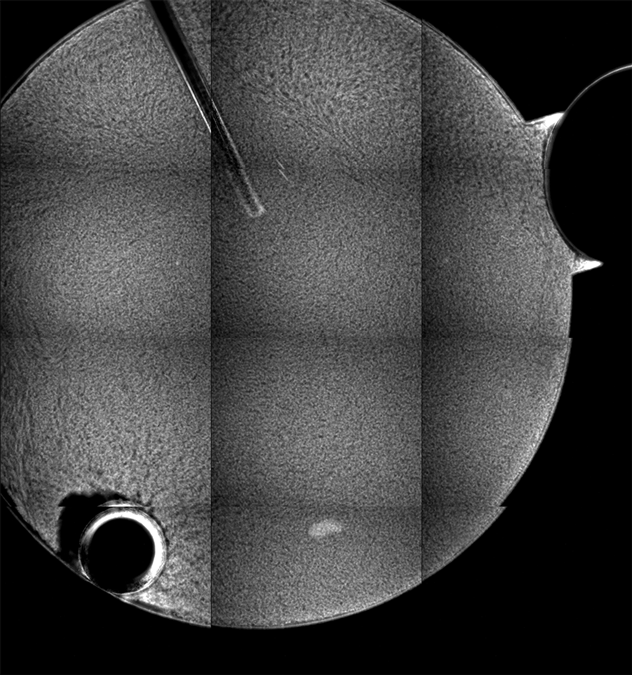
\includegraphics[width=\columnwidth]{./images/2014_07_27_ace_m2_run4_s22_gel/w9s22_10x_days02to15_resize.png}
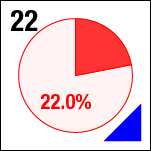
\includegraphics{./images/ace_m2_sample_tiles/sample22.png}
\caption{10x composite, raw images}
\end{center}
\end{figure}

The position shifts slightly, and the brightness changes. Clearly, the images
are not exactly aligned, and the motion distracts from being able to watch any
evolution in the sample, as well as interfering with any automated analysis.

\subsection{Pre-processing image
data}\hypertarget{pre-processing-image-data}{}\label{pre-processing-image-data} To fix these issues, I will align the images within the time sequence, and match
their brightnesses so that the intensity doesn't change so dramatically.

\subsubsection{Aligning the
images}\hypertarget{aligning-the-images}{}\label{aligning-the-images} The first major task is to align the images from subsequent days of data
collection. I first rename
the files, then in Photoshop CS6 import the set of images into separate layers
in a composite image, with {\tt File \textgreater{} Scripts \textgreater{} Load
Files into Stack...}, enabling the option to {\tt Attempt to Automatically Align
Source Images}. This works pretty well for these images, where the overall shape
of the well can guide the alignment algorithm.

This process is not fast, taking several seconds per image, but for just a
handful of images, it works well enough. By contrast, for BCAT, where we have
hundreds of frames, I create an image sequence movie in Adobe After Effects, and
use the tracking features there to far more quickly do the alignment.

I then crop the images so that there are no blank borders, and save the file as
a mult-layer {\tt .psd} file.

\subsubsection{Matching
intensities}\hypertarget{matching-intensities}{}\label{matching-intensities} For color images, the Photoshop feature {\tt Match Color...} is very good and
extremely helpful. In our case, however, grayscale images do not have the same
feature, and the option is unavailable. Instead, using a combination of {\tt
Levels} and ```Curves, I adjust each image to have the same mean (a little over
100 in 8-bit grayscale values) and standard deviation (about 60 8-bit grayscale
levels).

\subsubsection{Building the
animation}\hypertarget{building-the-animation}{}\label{building-the-animation} In the {\tt Timeline} palette, I {\tt Create Frame Animation}, then in the
drop-down menu select {\tt Make Frames from Layers}. The great thing about this
feature is that it otherwise doesn't affect anything about the image or its
layers. The final step is to export to an animated {\tt .gif} file, using the
{\tt Save for Web...} dialog box. There I reduce to final web resolution, and
create the final file:
\begin{figure}[h]
\begin{center}
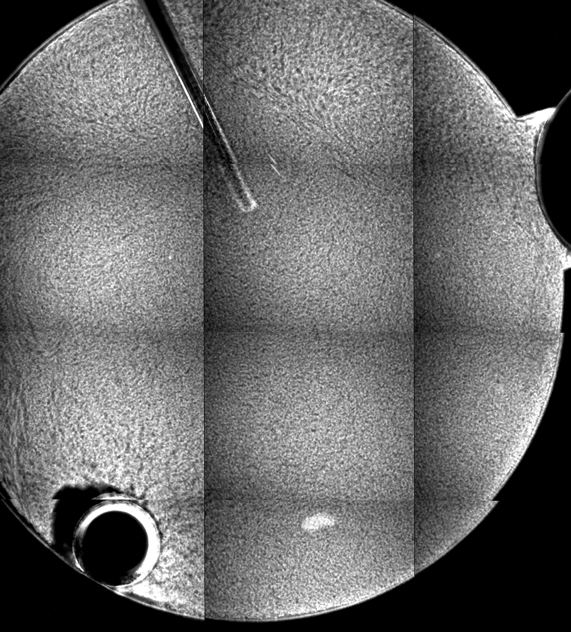
\includegraphics[width=\columnwidth]{./images/2014_07_27_ace_m2_run4_s22_gel/w9s22_10x_days02to15.png}
\end{center}
\caption{10x composite, aligned images}
\end{figure}

\clearpage

\subsection{Higher
magnification}\hypertarget{higher-magnification}{}\label{higher-magnification} I apply the same procedure to the higher-magnification 40x composite. First, the
raw data (just resized):
\begin{figure}[h]
\begin{center}
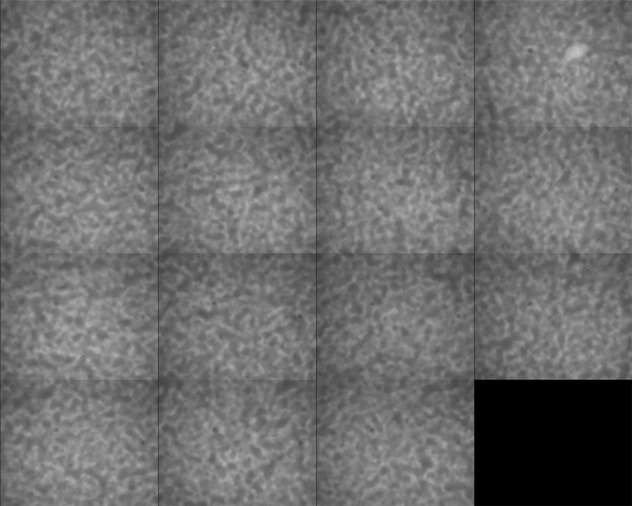
\includegraphics[width=\columnwidth]{./images/2014_07_27_ace_m2_run4_s22_gel/w9s22_40x_60um_days04to15_resize.png}
\end{center}
\caption{40x composite, raw images}
\end{figure}

And then the corrected version, where the aligned images have a mean of 128 and standard deviation of 40 8-bit grayscale levels:
\begin{figure}[h]
\begin{center}
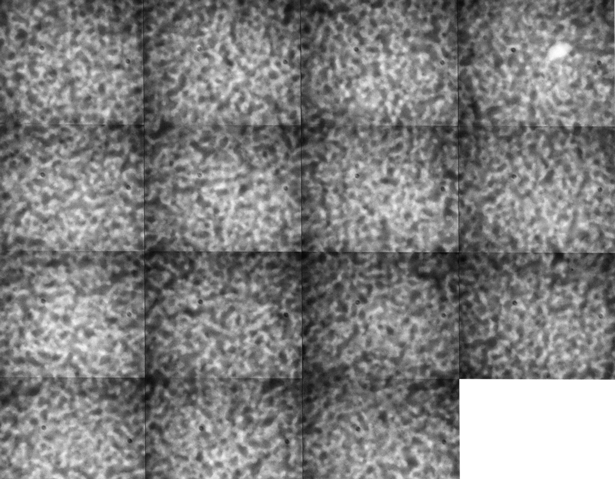
\includegraphics[width=\columnwidth]{./images/2014_07_27_ace_m2_run4_s22_gel/w9s22_40x_60um_days04to15.png}
\end{center}
\caption{40x composite, aligned images}
\end{figure}

%\subsection{Stage reproducibility or drift?}
Several things are apparent from these sequences. First, the stage is not
perfectly reproducible from a mechanical standpoint. The composites seem to move
around a little bit, likely due to mechanical backlash in the stage. Second,
intensities are not constant from day to day.
\end{document}